%!TEX root = research_proposal.tex

\chapter{Background \& Related Work\label{chap:relwork}}

In this chapter we present preliminaries in Section \ref{sec:preliminaries}.
These preliminaries describe the set of definitions we are using as same as project and versioning systems.
Then, we present related works for crash reproduction, crash prediction, linking report and source code modifications and clone detection.

\section{Preliminaries\label{sec:preliminaries}}

Software maintenance, comprehension, evolution, specifications and testing are research areas overlapping each other in terms of terminology.

In this proposal, we will use a precise set of definitions.
We do not claim ownership of these definitions, they have been established using various resources \cite{Avizienis2004,Pratt2001,Burnstein2006,Radatz1990,Whittaker2012}.

We limit software maintenance to the following three artifacts:

\begin{itemize}
	\item Bug report: A bug report describes a behavior observed in the field and considered abnormal by the reporter. Bug reports are submitted manually to bug report systems (bugzilla/jira). There is no mandatory format to report a bug, nevertheless, it should have: Version of the software / OS / Platform used, steps to reproduce, screen shots, stack trace and anything that could help a developer to assess the internal state of the software system.
	\item Crash report: A crash report is the last action a software system does before crashing. Crash reports are automatic (they have to be implemented into the software system by developer) and contain data (that can be proprietary) to help developers understand the crash (e.g. memory dump,...).
	\item Tasks: A task is a new feature, or the improvement of an existing feature, to be implemented in a future release of the software.
\end{itemize}

These artifacts are produced in response to the following phenomena:

\begin{itemize}
	\item Software Bug: A software bug is an error, flaw, failure, defect or fault in a computer program or system that causes it to violate at least one of its functional or nonfunctional requirements.
	\item Error: An error is a mistake, misconception, or misunderstanding on the part of a software developer.
	\item Fault/defect: A fault (defect) is defined as an abnormal condition or defect at the component, equipment, or subsystem level which may lead to a failure. A fault (defect) is not final (the system still works) and does not prevent a given feature to be accomplished.  A fault (defect) is a deviation (anomaly) of the healthy system that can be caused by an error or external factors (hardware, third parties, ...).
	\item Failure: The inability of a software system or component to perform its required functions within specified requirements.
	\item Crash: The software system encountered a fault (defect) that triggered a fatal failure from which the system could not recover from/overcome. As a result,  the system stopped.
\end{itemize}

In the remaining of this section, we introduce the two types of software repositories: version control and project tracking system.

\subsection{Version control systems\label{sec:version-control}}

Version control consists of maintaining the versions of files --- such as source code and other software artifacts \cite{Zeller1997}.
This activity is a complex task and cannot be performed manually on real world project.
Consequently, numerous tools have been created to help practitioners manage the version of their software artifacts.
Each evolution of a software is a version (or revision) and each version (revision) is linked to the one before through modifications of software artifacts.
These modifications consist of updating, adding or deleting software artifacts.
They can be referred as \texttt{diff}, {\tt patch} or {\tt commit}\footnote{These names are not to be used interchangeably as difference exists.}.
Each \texttt{diff}, {\tt patch} or {\tt commit} have the following characteristics:

\begin{itemize}
\item Number of Files: The number of software files that have been modified, added or deleted.
\item Number of Hunks: The number of consecutive code blocks of modified, added or deleted lines in textual files. Hunks are used to determine, in each file, how many different places the developer has modified.
\item Number of Churns:  The number of lines modified. However, the churn value for a line change should be at least two as the line has to be deleted first and then added back with the modifications.
\end{itemize}

Modern version control systems also support branching.
A branch is a derivation in the evolution that contains a duplication of the source code so that both versions can be modified in parallel.
Branches can be reconciled with a merge operation that merge modification of the two branches.
This operation is completely automated at the exception of merging conflicts that arise when both branches contain modification of the same line.
Such conflicts cannot be reconciled automatically and have to be dealt with by the developer.
This allows for a greater agility among developers as changes on one branch do not affect other developers of other branches.

Branching have been used for more than testing hazardous refactoring or testing framework upgrades.
Indeed, task branching is an agile branching strategy where a new branch is created for each task \cite{MartinFowler2009}.
It is common to see branch named {\tt 123\_implement\_X} where {\tt 123} is the {\tt \#id} of task {\tt X} given by the project tracking system.
Project tracking systems are presented in Section \ref{sec:issue-tracking}.

In modern versioning systems, when maintainers make modifications to the source code want to version it, they have to do commit.
The commit operation will version the modifications applied to one or many files.

Figure \ref{fig:branching} presents the data structure used to store a commit.
Each commit is represented as a tree.
The root leaf (green) contains the commit, tree and parent hashes as same as the author and the description associated with the commit.
The second leaf (blue) contains the leaf hash and the hashes of the files of the project.

\begin{figure}[h!]
  \centering
    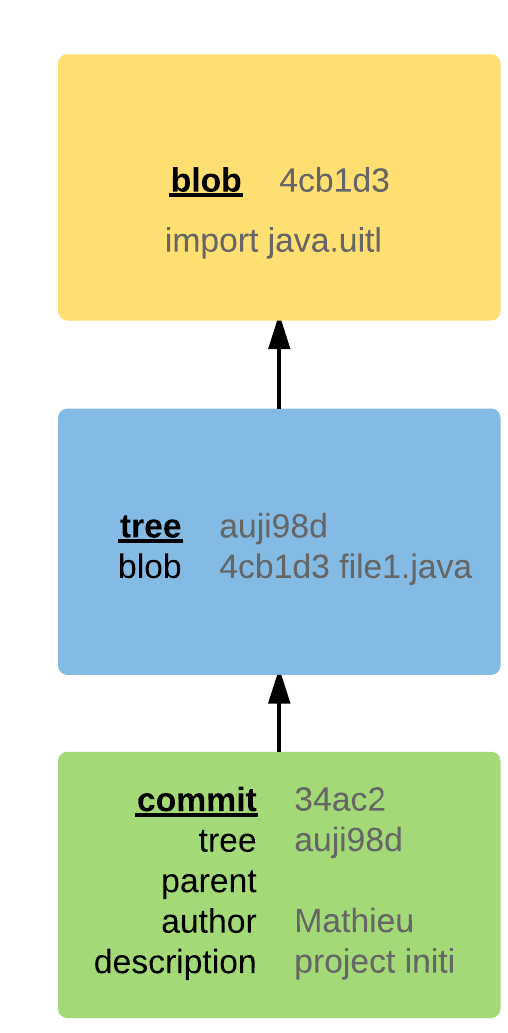
\includegraphics[scale=0.25]{media/commit-datastructure.png}
    \caption{Data structure of a commit.
    \label{fig:branching}}
\end{figure}

In this example, we can see that author ``Mathieu'' has created the file $file1.java$ with the message ``project init''.
Figure \ref{fig:two-commits} represents an ulterior modification.
In this second example, $file1. java$ is modified while $file2.java$ is created.
The second commit $98ca9$ have $34ac2$ as a parent.

\begin{figure}[h!]
  \centering
    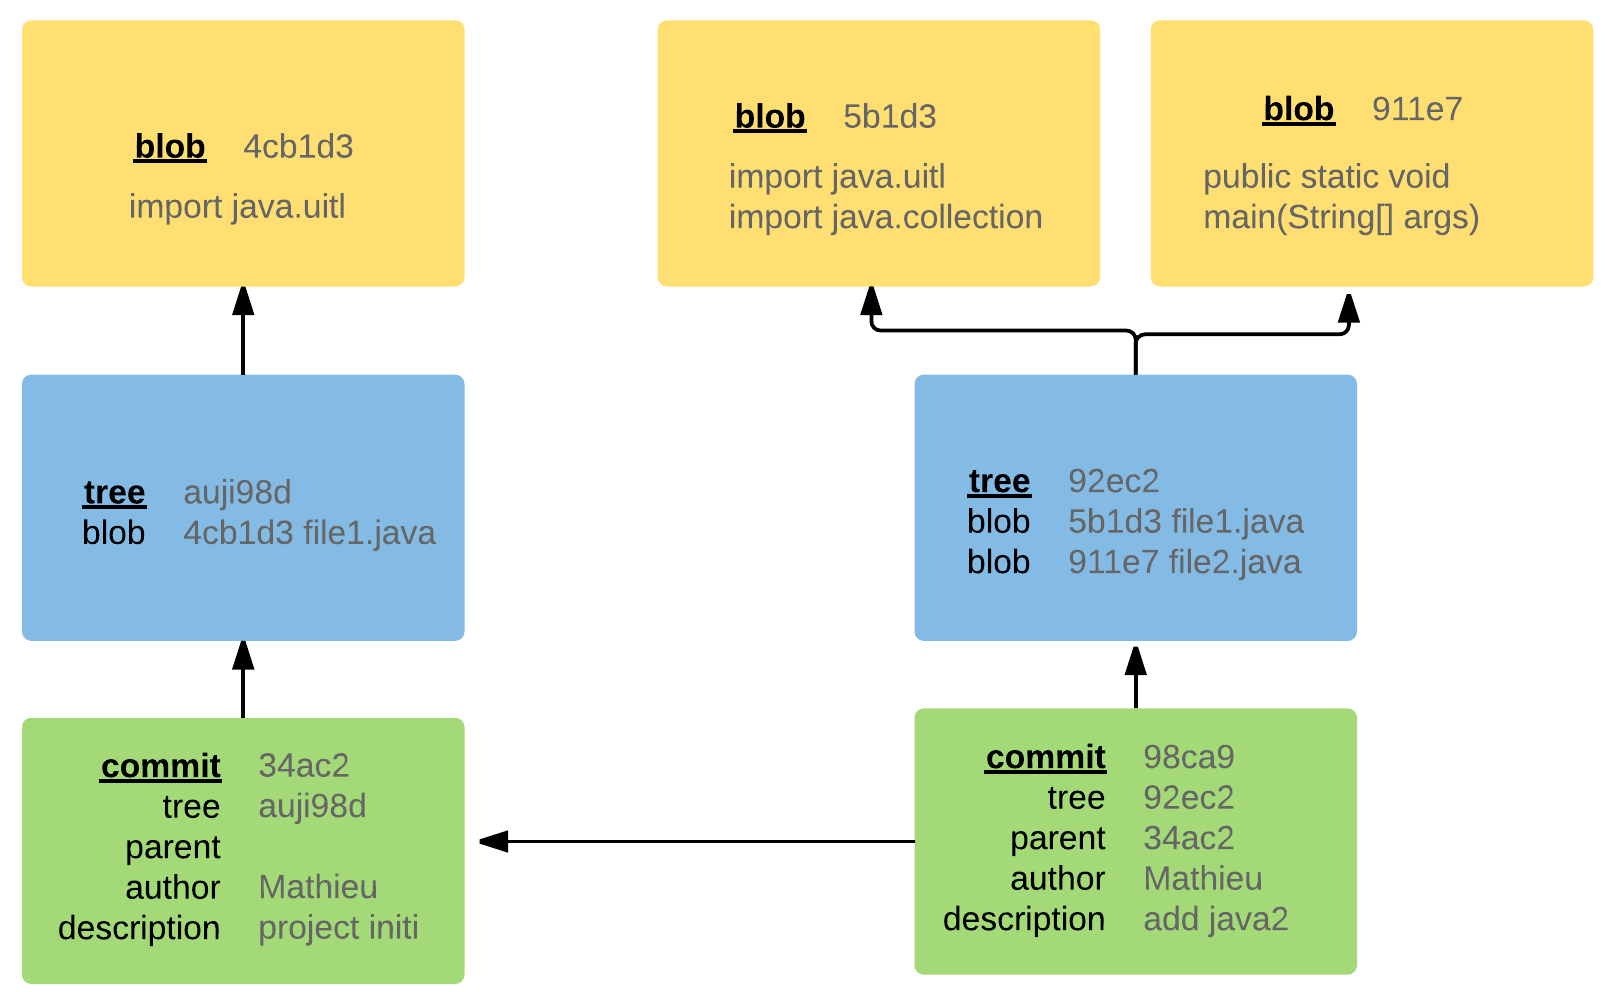
\includegraphics[scale=0.25]{media/branching.png}
    \caption{Data structure of two commits.
    \label{fig:two-commits}}
\end{figure}

Branches point to a commit.
In a task-branching environment, a branch is created via a checkout operation for each task.
Tasks can be to fix the root cause of a crash or bug report or features to implement.
In figure \ref{fig:two-branches}, the $master$ branch and the $1\_fix\_overflow$ point on commit $98ca9$.

\begin{figure}[h!]
  \centering
    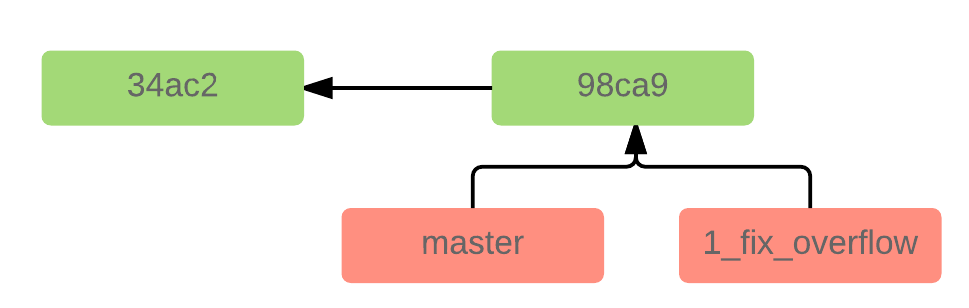
\includegraphics[scale=0.25]{media/2branches.png}
    \caption{Two branches pointing on one commit.
    \label{fig:two-branches}}
\end{figure}

Both branches can evolve separately and be merged together when the task branch is ready.
In figure \ref{fig:merge}, the $master$ branch points on $a13ab2$ while the $1\_fix\_overflow$ points on $ahj23k$.

\begin{figure}[h!]
  \centering
    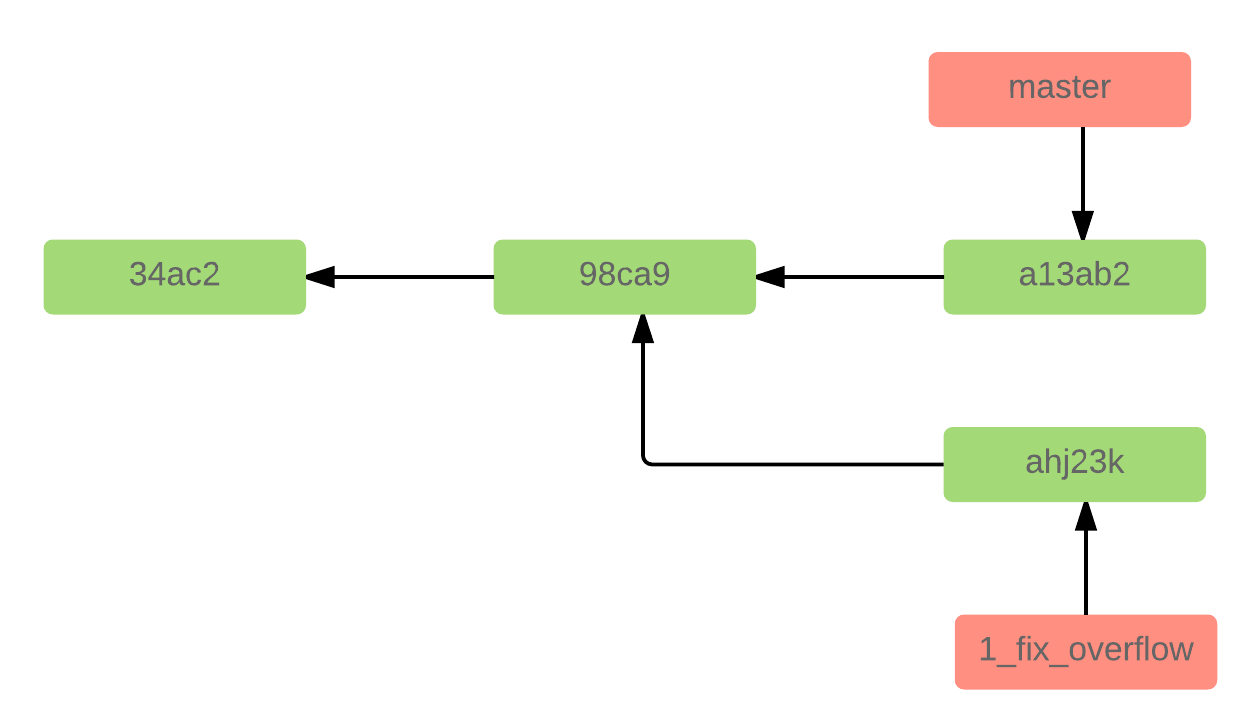
\includegraphics[scale=0.25]{media/merge.png}
    \caption{Two branches pointing on two commits.
    \label{fig:merge}}
\end{figure}


\subsubsection{Providers\label{sec:revision-provider}}

In this proposal, we mainly refer to three version control systems: {\tt Svn}, {\tt Git} and, to a lesser extent, {\tt Mercurial}.
{\tt SVN} is distributed by the Apache foundation and is a centralized concurrent version system that can handle conflict in the different versions of different developers and it is widely used.
At the opposite, {\tt Git} is a distributed revision control system --- originally developed by Linus Torvald --- where revisions can be kept locally for a while and then shared with the rest of the team.
Finally {\tt Mercurial} is also a distributed revision system, but share a lot of concepts with {\tt Svn}.
Consequently, it will be easier for people used to {\tt Svn} to switch to a distributed revision system if they use {\tt Mercurial}.

\subsection{Project Tracking Systems\label{sec:issue-tracking}}

Project tracking systems allow end users to create bug reports (BRs) to report unexpected system behavior,
manager can create tasks to drive the evolution forward and crash report (CRs) can be automatically created.
These systems are also used by development teams to keep track of the modification induced by bug and to crash reports, and keep track of the fixes.


\begin{figure}[h!]
	\centering
	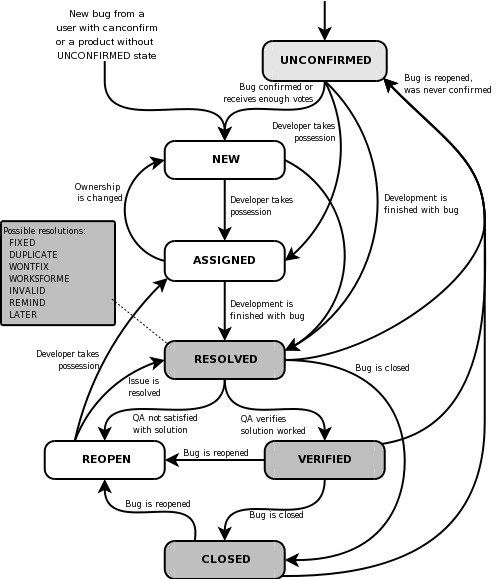
\includegraphics[scale=0.7]{media/bzLifecycle.png}
	\caption{Lifecyle of a report \cite{Bugzilla2008}}
	\label{fig:bug-lifecyle}
\end{figure}

Figure \ref{fig:bug-lifecyle} presents the life cycle of a report.
When a report is submitted by an end-user, it is set to the {\tt UNCONFIRMED} state until it receives enough votes or that a user with the proper permissions modifies its status to {\tt NEW}.
The report is then assigned to a developer to be fixed.
When the report is in the {\tt ASSIGNED} state, the assigned developer(s) starts working on the report.
A fixed report moves to the {\tt RESOLVED} state. Developers have five different possibilities to resolve a report: {\tt FIXED}, {\tt DUPLICATE}, {\tt WONTFIX}, {\tt WORKSFORME} and {\tt INVALID} \cite{Koponen2006}.

\begin{itemize}
	\item {\tt RESOLVED/FIXED}: A modification to the source code has been pushed, i.e., a changeset (also called a patch) has been committed to the source code management system and fixes the root problem described in the report.
	\item {\tt RESOLVED/DUPLICATE}: A previously submitted report is being processed. The report is marked as duplicate of the original report.
	\item {\tt RESOLVED/WONTFIX}: This is applied in the case where developers decide that a given report will not be fixed.
	\item {\tt RESOLVED/WORKSFORME}: If the root problem described in the report cannot be reproduced on the reported OS / hardware.
	\item {\tt RESOLVED/INVALID}: If the report is not related to the software itself.
\end{itemize}

Finally, the report is {\tt CLOSED} after it is resolved.
A report can be reopened (sent to the {\tt REOPENED} state) and then assigned again if the initial fix was not adequate (the fix did not resolve the problem).
The elapsed time between the report marked as the new one and the resolved status are known as the {\it fixing time}, usually in days.
In case of task branching, the branch associated with the report is marked as ready to be merged.
Then, the person in charge (quality assurance team, manager, ect...) will be able to merge the branch with the mainline.
If the report is reopened: the days between the time the report is reopened and the time it is marked again as {\tt RESOLVED/FIXED} are cumulated.
Reports can be reopened many times.

Tasks follow a similar life cycle with the exception of the {\tt UNCONFIRMED} and {\tt RESOLVED} states.
Tasks are created by management and do not need to be confirmed in order to be {\tt OPEN} and {\tt ASSIGNED} to developers.
When a task is complete, it will not go to the {\tt RESOLVED} state, but to the {\tt IMPLEMENTED} state.
Bug and crash reports are considered as problems to eradicate in the program.
Tasks are considered as new features or amelioration to include in the program.

Reports and tasks can have a severity\cite{Bettenburg2008}.
The severity is a classification to indicate the degree of  impact on the software.
The possible severities are:

\begin{itemize}
	\item blocker: blocks development and/or testing work.
	\item critical: crashes, loss of data, severe memory leak.
	\item major: major loss of function.
	\item normal: regular report, some loss of functionality under
 specific circumstances.
  \item minor: minor loss of function, or other problem where easy workaround is present.
	\item trivial: cosmetic problems like misspelled words or misaligned text.
\end{itemize}

The relationship between an report or a task and the actual modification can be hard to establish and it has been a subject of various research studies (e.g., \cite{Antoniol2002,Bachmann2010,Wu2011}).
This reason is that they are in two different systems: the version control system and the project tracking system.
While it is considered a good practice to link each report with the versioning system by indicating the report $\#id$ on the modification message, more than half of the reports are not linked to a modification\cite{Wu2011}.

\subsubsection{Providers\label{sec:bug-provider}}

We have collected and plan to collect data from four different project tracking systems: $Bugzilla$, $Jira$, $Github$ and $Sourceforge$.
 $Bugzilla$ belongs to the Mozilla foundation and has first been released in 1998.
 $Jira$, provided by Altassian, has been released 14 years ago, in 2002.
 $Bugzilla$ is 100\% open source and it's difficult to estimate how many project uses it.
 However, we can, without any risks envision that it owns a great share of the market as major organizations such as Mozilla, Eclipse and the Apache Software Foundation uses it.
 $Jira$, in the other hand, is a commercial software --- with a freemium business model --- and Altassian claims that they have 25,000 customers over the world.

$Github$ and $Sourceforge$ are different from $Bugzilla$ and $Jira$ in a sense that they were created as source code revision system and evolve, later on, to add project tracking capabilities to their softwares.
This common particularity have the advantage to ease the link between reports and source code.

\section{Crash reproduction\label{sec:rel-reproduction}}

The first (and perhaps main) step in understanding the cause of a field crash is to reproduce the bug that caused the system to fail.
A survey conducted with developers of major open source software systems such as Apache, Mozilla and Eclipse revealed that one of the most valuable piece of information that can help locate and fix the cause of a crash is the one that can help reproduce it \cite{Bettenburg2008}.

Crash reproduction is, however, a challenging task because of the limited amount of information  provided by the end users.
There exist several bug reproduction techniques. They can be grouped into two categories: (a) On-field record and in-house replay \cite{Narayanasamy2005,Artzi2008,Jaygarl}, and (b) In-house crash explanation \cite{Manevich2004,chandra2009snugglebug}.
The first category relies on instrumenting the system in order to capture objects and other system components at run-time.
When a faulty behavior occurs in the field, the stored objects, as well as the entire heap, are sent to the developers along with the faulty methods to reproduce the crash.
These techniques tend to be simple to implement and yield good results, but they suffer from two main limitations.
First, code instrumentation comes with a non-negligible overhead on the system.
The second limitation is that the collected objects may contain sensitive information causing customer privacy issues.
The second category is composed of tools leveraging proprietary data in order to provide hints on potential causes. While these techniques are efficient in improving our comprehension of the bugs, they are not designed with the purpose of reproducing them.

These two categories yield varying results depending on the selected approach and are mainly differentiated by the need for instrumentation.
The first category of techniques oversees --- by means of instrumentation --- the execution of the target system on the field in order to reproduce the crashes in-house, whereas tools and approaches belonging to the second category only use data produced by the crash such as the crash stack or the core dump at crash time.
In the first category, tools record different types of data such as the invoked methods \cite{Narayanasamy2005}, try-catch exceptions \cite{Rossler2013}, or objects \cite{Jaygarl}.
In the second category, existing tools and approaches are aimed towards understanding the causes of a crash, using data produced by the crash itself, such as a crash stack \cite{Chen2013a}, previous --- and controlled --- execution \cite{Zuddas2014}, etc.

Tools and approaches that rely on instrumentation face common limitations such as the need to instrument the source code in order to introduce logging mechanisms\cite{Narayanasamy2005,Jaygarl,Artzi2008}, which is known to slow down the subject system.
In addition,  recording system behavior by means of instrumentation may yield privacy concerns.
Tools and approaches that only use data about a crash --- such as core dump or exception stack crashes --- face a different set of limitations. They have to reconstruct the timeline of events that have led to the crash \cite{Chen2013a,Nayrolles2015}.
Computing all the paths from the initial state of the software to the crash point is an NP-complete problem, and may cause state space explosion \cite{Chen2013a,Clause2007}.

In order to overcome these limitations, some researchers have proposed to use various SMT (satisfiability modulo theories) solvers \cite{Dutertre2006} and model checking techniques \cite{Visser2003}.
However, these techniques require knowledge that goes beyond traditional software engineering, which hinders their adoption  \cite{Visser2004}.

It is worth mentioning that both categories share a common limitation.
It is possible for the required condition to reproduce a crash to be purely external such as the reading of a file that is only present on the hard drive of the customer or the reception of a faulty network packet \cite{Chen2013a, Nayrolles2015}.
It is almost impossible to reproduce the bug without this input.

\subsubsection{On-field Record and In-house Replay}

Jaygarl {\it et al.} created OCAT (Object Capture based Automated Testing) \cite{Jaygarl}.
The authors' approach starts by capturing objects created by the program when it runs on-field in order to provide them to an automated test process.
The coverage of automated tests is often low due to lack of correctly constructed objects. Also, the objects can be mutated by means of evolutionary algorithms.
These mutations target primitive fields in order to create even more objects and, therefore, improve the code coverage.
While not directly targeting the reproduction of a bug, OCAT is an approach that was used as the main mechanism for bug reproduction systems.

Narayanasamy {\it et al.} \cite{Narayanasamy2005} proposed BugNet, a tool that continuously records program execution for deterministic replay debugging.
According to the authors, the size of the recorded data needed to reproduce a bug with high accuracy is around 10MB.
This recording is then sent to the developers and allows the deterministic replay of a bug.
The authors argued that with nowadays Internet bandwidth the size of the recording is not an issue during the transmission of the recorded data.

Another approach in this category was  proposed by Clause {\it et al.} \cite{Clause2007}.
The approach records the execution of the program on the client side and compresses the generated data.
Moreover, the approach keeps compressed traces of all accessed documents in the operating system.
This data is sent to the developers to replay the execution of the program in a sandbox, simulating the client's environment.
This special feature of the approach proposed by Clause {\it et al.} addresses the limitation where crashes are caused by external causes.
While the authors broaden the scope of reproducible bugs, their approach records a lot of data that may be deemed private such as files used for the proper operation of the operating system.

Timelapse \cite{Burg2013} also addresses the problem of reproducing bugs using external data.
The tool focuses on web applications and allows developers to browse and visualize the execution traces recorded by Dolos. Dolos captures and reuses user inputs and network responses to deterministically replay a field crash.
Also, both Timelapse and Dolos allow developers to use conventional tools such as breakpoints and classical debuggers. Similar to the approach proposed by Clause {\it et al. \cite{Clause2007}}, private data are recorded without obfuscation of any sort.

Another approach was proposed by Artzi {\it et al.} and named ReCrash.
ReCrash records the object states of the targeted programs \cite{Artzi2008}.
The authors use an in-memory stack, which contains every argument and object clone of the real execution in order to reproduce a crash via the automatic generation of unit test cases.
Unit test cases are used to provide hints to the developers about the buggy code.
This approach particularly suffers from the limitation related to slowing down the execution.
The overhead for full monitoring is considerably high (between 13\% and 64\% in some cases).
The authors  propose an alternative solution in which they record only the methods surrounding the crash.
For this to work, the crash has to occur at least once so they could use the information causing the crash to identify the methods surrounding it.
ReCrash was able to reproduce 100\% (11/11) of the submitted bugs.

Similar to ReCrash, JRapture \cite{Steven2000} is a capture/replay tool for observation-based testing.
The tool captures the execution of Java programs to replay it in-house.
To capture the execution of a Java program, the creators of JRapture used their own version of the Java Virtual Machine (JVM) and a lightweight, transparent capture process.
Using a customized JVM allows capturing any interactions between a Java program and the system including GUI, files, and console inputs.
These interactions can be replayed later  with exactly the same input sequence as seen during the capture phase.
However, using a custom JVM is not a practical solution.
This is because, the authors' approach requires from users to install a JVM that might have some discrepancies with the original one and yield bugs if used with other software applications.
In our view,  JRapture fails to address the limitations caused by instrumentation because it imposes the installation of another JVM that can also monitor other software systems than the intended ones.
RECORE (REconstructing CORE dumps) is a tool proposed by Robler {\it et al.}.
The tool instruments Java byte code to wrap every method in a try-catch block while keeping a quasi-null overhead \cite{Rossler2013}.
RECORE starts from the core dump and tries (with evolutionary algorithms) to reproduce the same dump by executing the subject program many times.
When the generated dump matches the collected one, the approach has found the set of inputs responsible for the failure and was able to reproduce 85\% (6/7) of the submitted bugs.

The approaches presented at this point operate at the code level.
There exist also techniques that focus on recording user-GUI interactions \cite{Herbold2011,Roehm2015}.
Roehm {\it et al.} extract the recorded data using delta debugging \cite{Zeller2002}, sequential pattern mining, and their combination to reproduce between 75\% and 90\% of the submitted bugs while pruning 93\% of the actions.

Among the approaches presented here, only the ones proposed by Clause {\it et al.} and Burg {\it et al.} address the limitations incurred due to the need for external data  at the cost, however, of privacy.
To address the limitations caused by instrumentation,  the RECORE approach proposes to let users choose where to put the bar between the speed of the subject program, privacy, and bug reproduction efficiency.
As an example, users can choose to contribute or not to improving the software --- policy employed by many major players such as Microsoft in Visual Studio or Mozilla in Firefox --- and propose different types of monitoring where the cost in terms of speed, privacy leaks, and efficiency for reproducing the bug is clearly explained.

\subsubsection{On-house Crash Explanation}

On the other side of the picture, we have tools and approaches belonging to the on-house crash explanation  (or understanding), which are fewer but newer than on-field record and replaying tools.

Jin {\it et al.} proposed BugRedux for reproducing field failures for in-house debugging \cite{Jin2012}.
The tool aims to synthesize in-house executions that mimic field failures.
To do so, the authors use several types of data collected in the field such as stack traces, crash stack at points of failure, and call sequences.
The data that successfully reproduced the field crash is sent to software developers to fix the bug.
BugRedux relies on several in-house executions that are synthesized so as to narrow down the search scope,  find the crash location, and finally reproduce the bug.
However, these in-house executions have to be conducted before the work on the bug really begins.
Also, the in-house executions suffer from the same limitation as unit testing, {\it i.e.}, the executions are based on the developer's knowledge and ability to develop exceptional scenarios in addition to the normal ones.
Based on the success of BugRedux, the authors built F3 (Fault
localization for Field Failures) \cite{Jin2013} and MIMIC \cite{Zuddas2014}.
F3 performs many executions of a program on top of BugRedux in order to cover different paths leading to the fault.
It then generates many ``pass'' and ``fail'' paths, which can lead to a better understanding of the bug.
They also use grouping, profiling and filtering, to improve the fault localization process.
MIMIC further extends F3 by comparing a model of correct behavior to failing executions and identifying violations of the model as potential explanations for failures.

Likewise, Zamfir {\it et al.} proposed ESD \cite{Zamfir2010}, an execution synthesis approach that automatically synthesizes failure execution using only the stack trace information. However, this stack trace is extracted from the core dump and may not always contain the components that caused the crash.

To the best of our knowledge, the most complete work in this category is the one of Chen in his Ph.D thesis \cite{Chen2013a}.
Chen proposed an approach named STAR (Stack Trace based Automatic crash Reproduction).
Using only the crash stack, STAR starts from the crash line and goes backward towards the entry point of the program. During the backward process, STAR computes the required condition using an SMT solver named Yices \cite{Dutertre2006}.
The objects that satisfy the required conditions are generated and orchestrated inside a JUnit test case. The test is run and the resulting crash stack is compared to the original one.
If both match, the bug is said to be reproduced.
STAR aims to tackle the state explosion problem of reproducing a bug by reconstructing the events in a backward fashion and therefore saving numerous states to explore. STAR was able to reproduce 38 crashes out of 64 (54.6\%).
Also, STAR is relatively easy to implement as it uses Yices \cite{Dutertre2006} and potentially Z3 \cite{de2008z3} (stated in their future work) that are well-supported SMT solvers.

Except for STAR, existing approaches that target the reproduction of field crashes require the instrumentation of the code or the running platform in order to save the stack call or the objects to successfully reproduce crash.
As we discussed earlier, such approaches yield good results 37.5\% to 100\% but the instrumentation can cause a massive overhead (1\% to 1066\%) while running the system.
In addition, the data generated at run-time using instrumentation may contain sensitive information.

\section{Reports and source code relationships\label{rel:issue-rela}}

Mining bug repositories is perhaps one of the most active research fields today. The reason is that the analysis of bug reports (BRs) provides useful insight that can help with many maintenance activities such as bug fixing \cite{Weiß2007,Saha2014} bug reproduction \cite{Chen2013,Artzi2008,Jin2012}, fault analysis \cite{Nessa2008}, etc.
This increase of attention can be further justified by the emergence of many open source bug tracking systems, allowing software teams to make their bug reports available online to researchers.

These studies, however, treat all bugs as the same. For
example, a bug that requires only one fix is analyzed the same way as a bug that necessitates multiple fixes.
Similarly, if multiple bugs are fixed by modifying the exact same locations in the code, then we should investigate how these bugs are related in order to predict them in the future.

Researchers have been studying the relationships between the bug and source code repositories since more than two decades.
To the best of our knowledge the first ones who conducted this type of study on a significant scale were Perry and Stieg \cite{PerryDewayneE.1993}.
In these two decades, many aspects of these relationships have been studied in length.
For example, researchers were interested in improving the bug reports themselves by proposing guidelines \cite{Bettenburg2008}, and by further simplifying existing bug reporting models \cite{Herraiz2008}.

Another field of study consist of assigning these bug reports, automatically if possible, to the right developers during triaging \cite{Anvik2006,Jeong2009,Tamrawi2011a,Bortis2013}.
Another set of approaches focus on how long it takes to fix a bug \cite{Bhattacharya2011,Zhang2013,Saha2014} and where it should be fixed \cite{Zeller2013a,Zhou2012}.
With the rapidly increasing number of bugs, the community was also interested in prioritizing bug reports \cite{Kim2011c}, and in predicting the severity of a bug \cite{Lamkanfi2010}.
Finally, researchers proposed approaches to predict which bug will get reopened \cite{Zimmermann2012,Lo2013}, which bug report is a duplicate of another one \cite{Bettenburg2008a,Tian2012a,Jalbert2008} and which locations are likely to yield new bugs \cite{Kim2006,Kim2007a}.

In her PhD thesis \cite{Eldh2001}, Sigrid Eldh discussed the classification of trouble reports with respect to a set of fault classes that she identified.
Fault classes include computational logical faults, ressource faults, function faults, etc.
She conducted studies on Ericsson systems and showed the distributions of trouble reports with respect to these fault classes.
A research paper was published on the topic in \cite{Eldh2007}.
Hamill et al.\cite{Hamill2014} proposed a classification of faults and failures in critical safety systems.
They proposed several types of faults and show how failures in critical safety systems relate to these classes.
They found that only a few fault types were responsible for the majority of failures.
They also compare on pre-release and post-release faults and showed that the distributions of fault types differed for pre-release and post-release failures.
Another finding is that coding faults are the most predominant ones.

\section{Crash Prediction}

Predicting crash, fault and bug is very large and popular research area.
The main goal behind the plethora of papers is to save on manpower---being the most expensive resource to build software---by directing their efforts on locations likely to contain a bug, fault or crash.

There are two distinct trends in crash, fault and bug prediction in the papers accepted to major venues such as MSR, ICSE, ICSME and ASE:  history analysis and current version analysis.

In the history analysis, researchers extract and interpret information from  the system.
The idea being that the files or locations that are the most frequently changed are more likely to contain a bug.
Additionally, some of these approaches also assume that locations linked to a previous bug are likely to be linked to a bug in the future.

On the other hand, approaches using only the current version to predict bugs assume that the current version, i.e. its design, call graph, quality metrics and more, will trigger the appearance of the bug in the future.
Consequently, they do no require the history and only need the current source-code.

In the remaining of this section, we will describe approaches belonging to the two families.

\subsubsection{Change logs approaches}
\label{subs:Change logs approaches}

Change logs based approaches rely on mining the historical data of the application and more particularly, the source code \textit{diffs}.
A source code \textit{diffs} contains two versions of the same code in one file.
Indeed, it contains the lines of code that have been deleted and the one that has been added.
It is worth noting that, \textit{diffs} files do not represent the concept of modified line.
Indeed, a modified line will be represented by a deletion and an addition.
Researchers mainly use five metrics when dealing with \textit{diffs} files:

\begin{itemize}
  \item Number of files: The number of modified files in a given commit
  \item Insertions: The number of added lines
  \item Deletions: The number of deleted lines
  \item Churns: The number of deleted lines immediately followed by an insertion which give an approximation of how many lines have been modified
  \item Hunks: The number of consecutive blocks of lines. This gives an approximation of how many distinct locations have been edited to accomplish a unit of work.
\end{itemize}

Naggapan \textit{et al.} studied the churns metric and how it can be connected to the apparition of new defect in a complex software systems.
They established that relative churns are, in fact, a better metric than classical churn \cite{Nagappan} while studying Windows Server 2003.

Hassan, interested himself with the entropy of change, i.e. how complex the change is \cite{Hassan2009}.
Then, the complexity of the change, or entropy, can be used to predict bugs.
The more complex a change is, the more likely it is to bring the defect with it.
Hassan used its entropy metric, with success, on six different systems.
Prior to this work, Hassan, in collaboration with Holt proposed an approach that highlights the top ten most susceptible locations to have a bug using heuristics based on \textit{diffs} file metrics \cite{Hassan2005}.
Moreover, their heuristics also leverage the data of the bug tracking system.
Indeed, they use the past defect location to predict new ones.
The conclusion of these two approaches has been that recently modified and fixed locations where the most defect-prone compared to frequently modified ones.

Similarly to Hassan and Hold,  Ostrand \textit{et al.} predict future crash location by combining the data from changed and past defect locations \cite{Ostrand2005}.
The main difference between Hassan and Hold and Ostrand \textit{et al.} is that Ostrand \textit{et al.} validate their approach on industrial systems as they are members of the AT\&T lab while Hassan and Hold validated their approach on open-source systems.
This proved that these metrics are relevant for open-source and industrial systems.

Kim \textit{et al.} applied the same recipe and mined recent changes and defects with their approach named bug cache \cite{Kim2007a}.
However, they are more accurate than the previous approaches at detecting defect location by taking into account that is more likely for a developer to make a change that introduces a defect when being under pressure.
Such changes can be pushed to revision-control system when deadlines and releases date are approaching.

\subsubsection{Single-version approaches}

Approaches belonging to the single-version family will only consider the current version of the software at hand.
Simply put, they don't leverage the history of changes or bug reports.
Despite this fact, that one can see as a disadvantage compared to approaches that do leverage history, these approaches yield interesting results using code-based metrics.

Chidamber and Kemerer published the well-known CK metrics suite \cite{Chidamber1994} for object oriented designs and inspired Moha \textit{et al.} to publish similar metrics for service oriented programs \cite{Moha}.
Another famous metric suite for assessing the quality of a given software design is Briand's coupling metrics \cite{Briand1999a}.

The CK and Briand's metrics suites have been used, for example, by Basili \textit{et al.} \cite{Basili1996}, El Emam \textit{et al.} \cite{ElEmam2001},  Subramanyam \textit{et al.} \cite{Subramanyam2003} and Gyimothy \textit{et al.} \cite{Gyimothy2005} for object oriented designs.
Service oriented designs have been far less studied than object oriented design as they are relatively new, but, Nayrolles \textit{et al.} \cite{Nayrolles,Nayrolles2013d}, Demange \textit{et al.} \cite{demange2013} and Palma \textit{et al.} \cite{Palma2013} used Moha et \textit{et al.} metric suites to detect software defects.

All these approaches, proved software metrics to be useful at detecting software fault for object oriented and service oriented designs, respectively.

Finally, Nagappan \textit{et al.} \cite{Nagappan2005,Nagappan2006} and Zimmerman \cite{Zimmermann2007,Zimmermann2008} further refined metrics-based detection by using statical analysis and call-graph analysis.

While hundreds of bug prediction papers have been published by academia over the last decade, the developed tools and approaches fail to change developer behavior while deployed in industrial environment \cite{Lewis2013}.
This is mainly due to the lack of actionable message, i.e. messages that provide concrete steps to resolve the problem at hand.

\section{Clone Detection}
\label{sec:rel-clones}

Some of our contributions rely on code clone detection to perform their functionalities.
Consequently, we reviewed the litterature of the field.
These section describes major works in clone detection.

Code clones appear when developers reuse code with little to no modification to the original code.
Studies have shown  that clones can account for about 7\% to 50\% of code in a given software system\cite{Baker, StephaneDucasse}.
Developers often reuse code (and create clones) in their software on purpose\cite{Kim2005}.
Nevertheless, clones are considered a bad practice in software development since they can introduce new bugs in the code\cite{Kapser2006,Juergens2009,Li2006}.
If a  bug is discovered in one segment of the code that has been copied and pasted several times, then the developers will have to remember the places where this segment has been reused in order to fix the bug in each place.

In the last two decades, there have been many studies and tools that aim at detecting clones.
They can be grouped into three categories.
The first category includes techniques that treat the source code as text and use transformation and normalization methods to compare various code fragments\cite{Johnson1994,Johnson1993, Cordy2011, Roy2008}.
The second category includes methods that use lexical analysis, where the source code is sliced into sequences of tokens, similar to the way a compiler operates\cite{Baker,Bakera,Baker2002,Kamiya2002,Li2006}.
The tokens are used to compare code fragments.
Finally, syntactic analysis has also been performed where the source code is converted into trees, more particularly abstract syntax tree (AST), and then the clone detection is performed using tree matching algorithms\cite{Baxter1998, Komondoor2000, Tairas2006, Falke2008}.

Although these techniques and tools have been shown to be useful in detecting clones, they operate in an offline fashion (i.e., after the clones have been inserted).
Software developers might be reluctant to use these tools on a day-to-day basis (i.e., as part of the continuous development process), unless they are involved in a major refactoring effort.
Johnson et al. \cite{Johnson2013} showed that these tools are challenging to use because they do not integrate well with the day-to-day workflow of a developer.
Also they output a large amount of data when applied to the entire system, making it hard to understand and analyse their results.

Text-based techniques use the code --- often raw (e.g. with comments) --- and compare sequences of code (blocks) to each other in order to identify potential clones. Johnson was perhaps the first one to use fingerprints to detect clones\cite{Johnson1993,Johnson1994}. Blocks of code are hashed, producing fingerprints that can be compared.
If two blocks share the same fingerprint, they are considered as clones.
Manber et al. \cite{Manber1994} and Ducasse et al.\cite{Ducasse1999} refined the fingerprint technique by using leading keywords and dot-plots.

Tree-matching and metric-based are two sub-categories of syntactic analysis for clone detection.
Syntactic analysis consists of building abstract syntax trees (AST) and analyse them with a set of dedicated metrics or searching for identical sub-trees.
Many approaches using AST have been published using sub-tree comparison including the work of Baxter et al.\cite{Baxter1998}, Wahleret et al. \cite{Wahler}, or more recently, the work of Jian et al. with Deckard \cite{Jiang2007}.
An AST-based approach compares metrics computed on the AST, rather than the code itself, to identify clones \cite{Patenaude1999, Balazinska}.

Another approach to detect clones is to use static analysis and to leverage the semantics of the program to improve the detection.
These techniques rely on program dependency graphs where nodes are statements and edges are dependencies.
Then, the problem of finding clones is reduced to the problem of finding identical sub-groups in the program dependency graph.
Examples of recent techniques that fall into this category are the ones presented by Krinke et al.\cite{Krinke2001} and  Gabel et al. \cite{Gabel2008}.

Many clone detection tools have been created using a lexical approach for clone detection. Here, the code is transformed into a series of tokens. If sub-series repeat themselves, it means that a potential clone is in the code. Some popular tools that use this technique include, but not limited to, Dup\cite{Baker}, CCFinder\cite{Kamiya2002}, and CP-Miner\cite{Li2006}.

Furthermore, a large number of taxonomies have been published in an attempt to classify  clones and ease the research on clone detection\cite{Mayrand1996,Balazinska1999,Koschke2006,Bellon2007,Kontogiannis,Kapser}.

Other active research activities in clone detection focus on clone removal and management.
Once detected, an obvious step is to provide approaches to remove clones in an automatic way or (at least) keep track of them if removing them is not an option.
Most modern IDEs provide the \textit{extract method} feature that transforms a potentially copy-pasted block of code into a method and a call to the newly generated method\cite{Komondoor,higo2004refactoring}.
More advanced techniques (see Codelink\cite{Toomim} and\cite{Duala-Ekoko2007}) involve analysing the output of CCFinder\cite{Kamiya2002a,Livieri2007} or program dependencies graphs\cite{higo2004refactoring} to automatically suggest a method that would go through the \textit{extract method} process.

The aforementioned  techniques, however, focus on detecting clones after they are inserted in the code. Only a few studies focus on preventing the insertion of clones. Lague et al. \cite{Lague} conducted a very large empirical study with 10,000 developers over 3 years, where developers where asked to use clone detection tools during the development process of a very large telecom system. The authors found that while clones are being removed over time, using clone detection tools help improving the quality of the system as it prevents defects to reach the customers. Duala et al. \cite{Duala-Ekoko2007,Duala-Ekoko2010} proposed to create clone region descriptors (CRDs), which describe clone regions within methods in a robust way that is independent from the exact text of the clone region or its location in a file. Then, using CRDs, clone insertion can be prevented.
